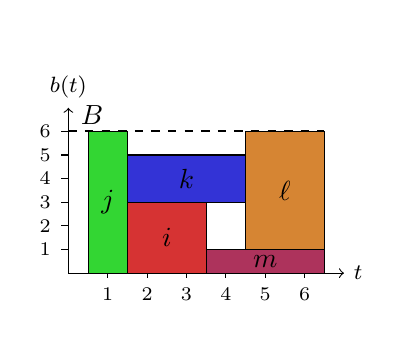
\begin{tikzpicture}
  [yscale=0.3, xscale= 0.5]
  \node at (0,10) {};

  \node[label={[shift={(-0.4,-0.5)}]}] (O) at (0,0) {};
  \draw[fill=red!80!black!80] (1.5,0) rectangle (3.5,3)   node[midway] {$i$};
  \draw[dashed,thick] (0,6)   -- (6.5,6);
  \node at (0.6,6.7)  {$B$};

  \draw[fill=green!80!black!80] (0.5,0) rectangle (1.5,6)   node[midway] {$j$};
  \draw[fill=blue!80!black!80] (1.5,3) rectangle (4.5,5)   node[midway] {$k$};
  \draw[fill=orange!80!black!80] (4.5,1) rectangle (6.5,6)   node[midway] {$\ell$};
  \draw[fill=purple!80!black!80] (3.5,0) rectangle (6.5,1)   node[midway] {$m$};

  
  \draw[->] (O.center) -- (0,7) node[above] {\footnotesize $b(t)$};
  \draw[->] (O.center) -- (7,0) node[right] {\footnotesize $t$};

  \foreach \i in {1,...,6}{
    \draw (0,\i) -- (-0.2,\i) node[left] {\scriptsize \i};
    \draw (\i, 0) -- (\i,-0.2) node[below] {\scriptsize \i};
}

\end{tikzpicture}
